% TEX root /home/nicholas/Scrivania/Obsidian/Secondo Anno/Secondo Semestre/APS - Analisi e Progettazione del Software/Latex/main.tex
\section{Cosa è l'Architettura Logica?}
L'architettura logica di un sistema software è l'organizzazione su larga scala delle classi software in package (o namespace), sottoinsiemi e strati.

È chiamata architettura logica poichè non vengono prese decisioni su come questi elementi siano distribuiti sui processi o sui diversi computer fisici di una rete

\section{Definizione di Architettura a Strati}
È uno stile di Architettura Logica in cui il sistema è formato da un insieme di elementi chiamati strati.

Ogni strato è un gruppo a grana molto grossa di classi, package o sottosistemi.

\subsection{Oraganizzazione degli strati}
Gli strati sono organizzati in modo tal che stati "più alti ricorrano ai servizi degli strati "più bassi"

\begin{figure}[H]
    \centering
    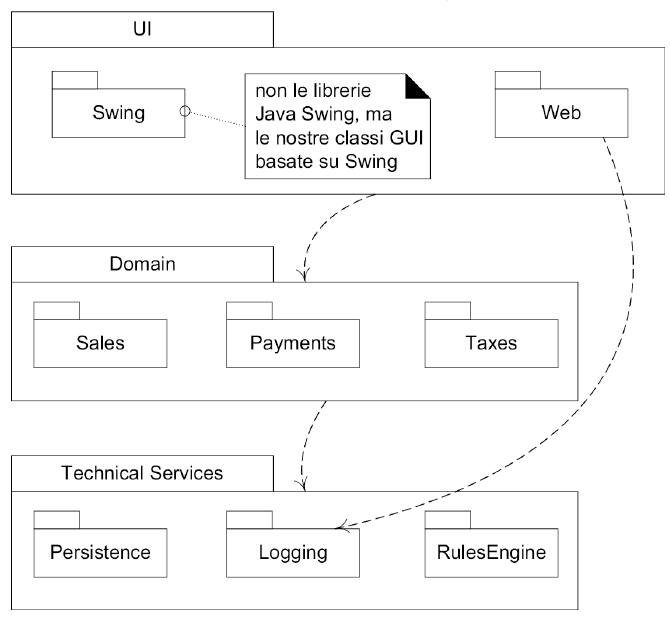
\includegraphics[scale=0.5]{figures/Schermata_20260428_113522}
    \caption{Strati mostrati con la notazione di un diagramma dei package di UML}
\end{figure}

\subsubsection{Architettura a stati stretta}
Uno strato può solo richiamare i servizi dello stato immediatamente sottostante
\subsubsection{Architettura a strati rilassata}
Uno strato pù alto può richiamare i servizi degli stati più bassi di diversi livelli

\subsection{Definizione degli strati}

Gli stati di un'applicazione software comprendono normalmente i seguenti

\subsubsection{User Interface}
Oggetti software per gestire l'interazione con l'utente e per la gestione degli eventi

\subsubsection{Application Logic e Domain Objects}
Oggetti software che rappresentano concetti del dominio (per esempio una classe software \texttt{Vendita}) che soddisfano i requisiti dell'applicazione

\subsubsection{Technical Services}
Oggetti e sottosistemi d'uso generale che forniscono servizi tecnici di supporto (Come l'accesso ai database o il logging degli errori)

\subsection{Progettazione degli stati}
L'obiettivo è organizzare la struttura logica del sistema in strati separati, ciascuno con responsabilità distinte e correlate.


Si attua una separazione netta :
\begin{itemize}
    \item Gli \textbf{strati inferiori} offrono servizi generali e di basso livello
    \item Gli \textbf{strati superiori} sono èiù specifici per l'applicazione
\end{itemize}
\subsection{Vantaggi dell'uso degli strati}
L'architettura a strati garantisce una netta separazione degli interessi tra i servizi specifici di alto livello e quelli generali di basso livello

\vspace{\baselineskip}
I vantaggi principali includono :
\begin{itemize}
    \item \textbf{Riduzione dell'accoppiamento }e delle dipendenze
    \item \textbf{Aumoneto della coesione, della chiarezza e del riuso}
    \item \text{Incapsulazione e decomposizione della complessità}
    \item Possibilità di \textbf{sostituire interi strati} con nuove implementazioni senza intaccare il resto del sistema
    \item Maggiore facilità nello \text{sviluppo da parte di più team}, grazie alla netta segmentazione logica
    \item Possibilità di distribuire alcuni strati su architetture fisiche diverse
\end{itemize}
\subsection{Reaponsabilità coese e separazione degli interessi}
All'interno di ciascun strato, le responsabilità degli oggetti devono essere fortemente coese tra loro e non devono mai essere mescolato con le responsabilità di altri strati

\section{Cosa è un'Architettura Software?}
Un architettura software riguarda l'organizzazione su larga scala del sistema.

Nello specifico essa è definita come :

\begin{itemize}
    \item L'insieme delle \textbf{decisioni significative} sull'organizzazione di un sistema software
    \item La \textbf{scelta degli elementi strutturali} da cui è composto il sistema e delle relative interfacce
    \item Il \textbf{comporamento} specificato dalla collaborazione tra questi elementi
    \item La \textbf{composizione} di questi elementi strutturali e comportamentali in sottosistemi via via più ampi
    \item Lo \textbf{stile architetturale} che fa da guida a questa organizzazione (come ad esempio l'architettura a strati)
\end{itemize}

\section{Diagrammi dei Package UML}
L'architettura logica di un sistema può essere illustrata mediante un diagramma dei package di UML
\subsection{Elementi dei diagrammi package}
\begin{itemize}
    \item Uno \textbf{strato} può essere modellato come un \textbf{packege UML}
    \begin{figure}[H]
        \centering
        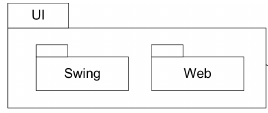
\includegraphics{figures/Schermata_20260428_141936.png}
        \caption{Strato di un architettura rappresentato come package UML}
    \end{figure}

    Uno package UML può raggruppare qualunque cosa (classi, altri package, casi d'uso)
    \item Una \textbf{dipendenza UML} è una linea tratteggiata con una freccia che punta verso il package da cui dipende

    \begin{figure}[H]
        \centering
        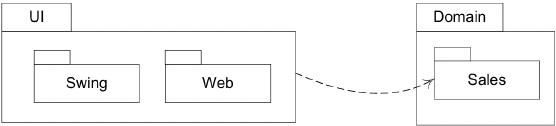
\includegraphics{figures/Schermata_20260428_142352.png}
        \caption{Esempio di uso di una dipendenza}
    \end{figure}
    \item Un package UML rappresenta un \textbf{namespace} cosicchè è possibile definire due classi con lo stesso nome su package diversi
\end{itemize}

\subsection{Definizione : Livelli, Strati e Partizioni}
\begin{figure}[H]
    \centering
    
\includegraphics{Schermata_20260428_151441.png}
\end{figure}
\begin{itemize}
    \item \textbf{Livello (tier)}

    Indica solitamente un nodo fisico di elaborazione
    \item \textbf{Strato (layer)}

    Rappresenta una sezione verticale dell'architettura logica
    \item \text{Partizione (partition)} 

    È una divisione orizzontale di un sottosistema posizionato all'interno di uno strato
\end{itemize}
